\section{Testbench}

The testbench was implemented using cocotb and verilator using a Makefile. The testbenches were used to verify 3 different levels of functionality:

\begin{enumerate}
    \item The UART receiver can receive data from the host.
    \item The UART controller can successfully transfer data from the UART to the instruction memory once the FIFO is full.
    \item The core can execute a program loaded in the instruction memory that was transferred from the UART FIFO.
\end{enumerate}

\begin{figure}[H]
    \centering
    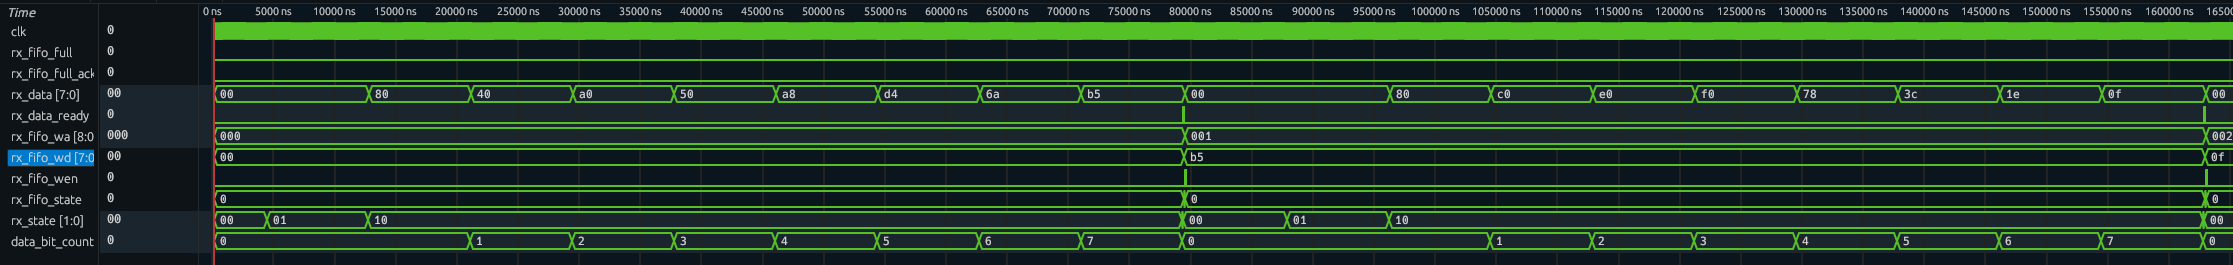
\includegraphics[width=\textwidth]{media/uart_rx}
    \caption{UART receiver waveform}
    \label{fig:uart_rx}
\end{figure}

For the first case, the waveform is shown in \autoref{fig:uart_rx}.
Here, the sent bytes were 0xB5 and 0x0F, which is confirmed by the \texttt{rx\_fifo\_wd} signal.

\begin{figure}[H]
    \centering
    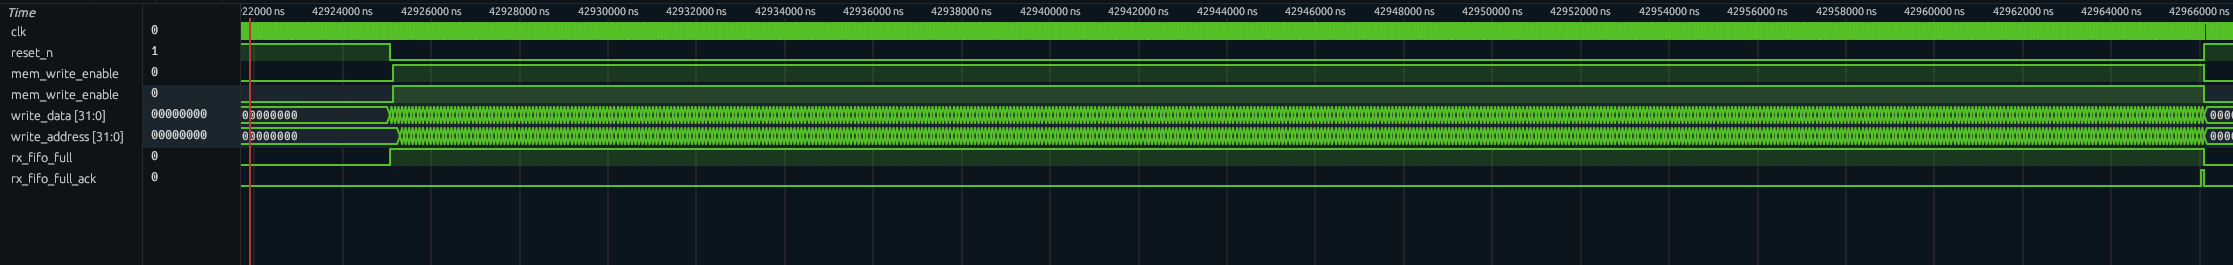
\includegraphics[width=\textwidth]{media/uart_full_fifo}
    \caption{UART full FIFO waveform}
    \label{fig:uart_full_fifo}
\end{figure}

\begin{figure}[H]
    \centering
    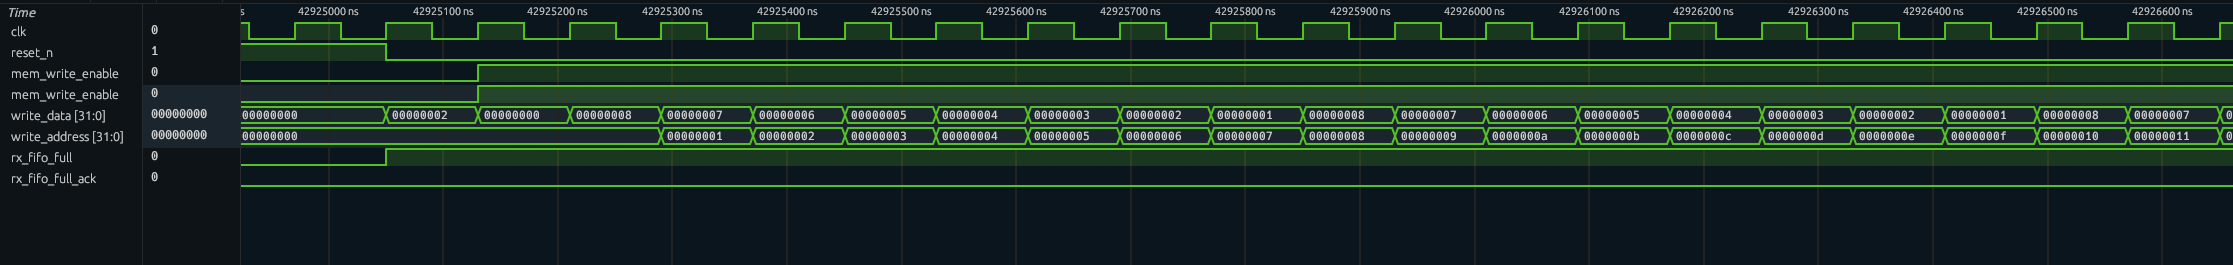
\includegraphics[width=\textwidth]{media/uart_full_fifo_zoomed}
    \caption{UART full FIFO waveform zoomed in}
    \label{fig:uart_full_fifo_zoomed}
\end{figure}

For the second case, the waveform is shown in \autoref{fig:uart_full_fifo}.
It successfully transfers the data from the UART FIFO to the instruction memory when the FIFO is full.
You can see that while the reset line is asserted low, the memory write enable signal is high and the \texttt{rx\_fifo\_full\_ack} is toggled at the end of the transfer.
In \autoref{fig:uart_full_fifo_zoomed}, you can see the write address incrementing as the memory is being written to.

\begin{figure}[H]
    \centering
    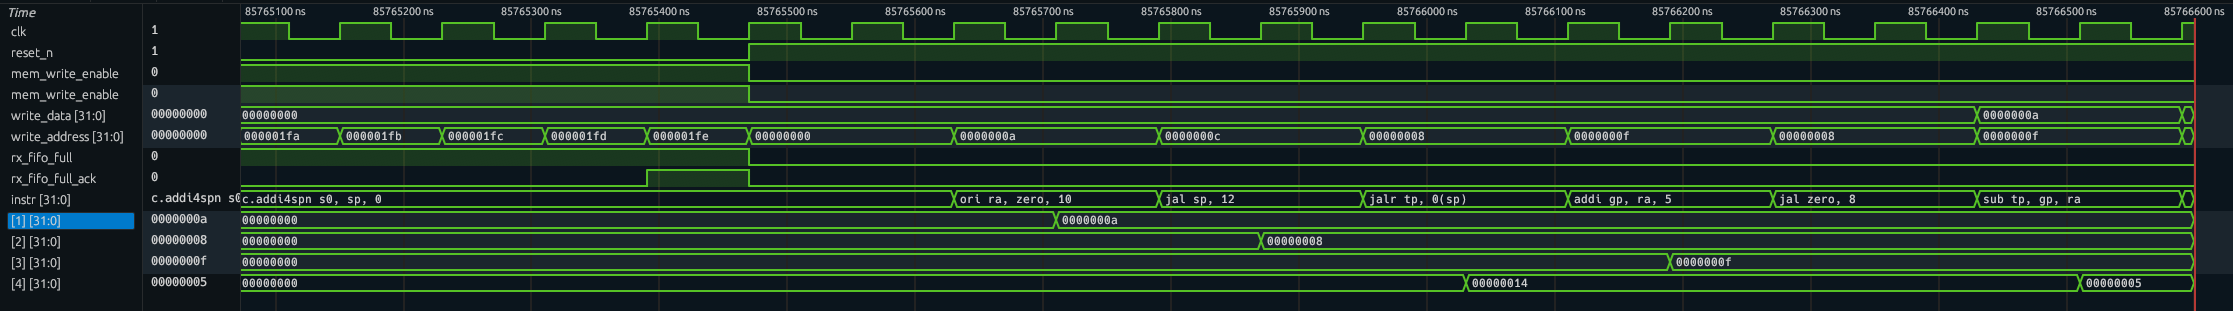
\includegraphics[width=\textwidth]{media/uart_reprogram}
    \caption{UART reprogram waveform}
    \label{fig:uart_reprogram}
\end{figure}

For the third case, the waveform is shown in \autoref{fig:uart_reprogram}.
After successfully transferring the program via UART, then to the instruction memory, the core comes out of reset when the FIFO full ack signal is toggled, and begins executing the loaded program.
The register contents shown in the waveform matches the expected results.